Though the line-integrated metastable densities are one of only a few
measurements made in the development of the \acs{rpnd}, they only provide a
limited view of what is happening. In addition to the metastables are ions,
electrons, a vast array of other excited states, and the electric fields. In an
effort to expand on the details of what is occurring within the \acs{rpnd}, it
is desirable to develop a model which can infer other properties from the
metastable measurements. This is possible, because the electrons which gain
energy from the electric fields are those which excite the metastables, other
excited states, and ions. The ideal model would solve the Boltzmann equation
(equation~\ref{eq:boltzmann}) for each species, over the entire geometry, in all
dimensions, for as long as was required to reach equilibrium.

Unfortunately, these requirements are somewhat problematic. Scale lengths of 10
$\mu$m are required in order to resolve the sheath effects, resulting in
approximately $2\times10^{13}$ spatial cells. Conservatively, the time steps
would be about 1 ns in length. At a minimum, the system required about five
minutes to reach equilibrium, thus necessitating $3\times10^{11}$ solution
steps. The largest velocity can be estimated as an electron accelerated across
the full applied potential (6.6 keV), and the lowest velocity would be room
temperature (0.04 eV). This produces a velocity discretization of about
$6\times10^7$ cells. Thus the size of the parameter space in question is about
$3.6\times10^{32}$. Given that the fastest computer in the world operates at 39
petaflops, a calculation of this magnitude would take around 0.3 billion years.
Of course, this is for only a single particle species, the total number in the
system is runs in the dozens (not including the impurities).

\section{Model Development}

It should be apparent that the Boltzmann equation must be simplified in order to
model the system in a reasonable amount of time. As discussed in
chapter~\ref{chp:theory}, the most common approach to this is the use of moments
of the Boltzmann equation which drastically simplifies the velocity terms.
Frequently, the moments of the Boltzmann equation are used to develop various
fluid approximations for plasmas \cite{Chen1984} (e.g.\ the two fluid equations,
the magnetohydrodynamic equations, etc.). This approach has been tremendously
successful in the description of everything from plasma display panels
\cite{Rauf1999b} to interstellar plasmas \cite{Linde1998}.

There are some limitation to the capabilities of these fluid descriptions. For
one, they require some assumption on the form of the \acs{eedf}. Often, the
distribution is assumed to be a Maxwell-Boltzmann or Druyvesteyn, depending on
the plasma conditions. In others, an approximate solution of the Boltzmann
equation may be used to tabulate rate coefficients as a function of the mean
energy \cite{Hagelaar2005}. In addition to this issue of the \acs{eedf}, fluid
models in large or complex geometries can still be quite computationally
expensive. This can limit the number of species and reactions which can be
addressed \cite{Lieberman2005}.

In order to obtain an estimate of the detailed dynamics which occur as the
\acs{rpnd} develops, it is necessary to consider additional simplifications of
the Boltzmann equation. One such possibility is the use of a global model where
the spatial dependence of the plasma parameters is assumed. This allows global
model simulations to ignore the geometry of the system and focus on the particle
interactions for long periods of time with reasonable computational
requirements.

Here, a global model will be developed to describe the evolution of the plasma
parameters along the measurement chords during the first pulse, and before the
reflection. As was seen in the metastable measurements, there was little axial
variation over the length of the discharge. Thus, as far as the model is
concerned, variations across the beam radius are negligible. However, it has
been noted that a similar \acs{fiw} \cite{Vasilyak1994} and the same \acs{rpnd}
\cite{Weatherford2012} exhibit radial variations in emission intensity, electron
density, and metastable density. Furthermore, these variations appear to depend
strongly on the operating pressure. Unfortunately, the cause of this is not
clearly understood, though it has been suggested that high-energy electrons from
the walls may be responsible \cite{Weatherford2012a}. Lacking any empirical,
theoretical, or numerical results that provide the evolution of the radial
profile during the discharge, it is necessary to assume one. In this case, the
plasma will be assumed to be uniform across the diameter of the discharge. This
assumption will affect the accuracy of the inferred plasma parameters, however
future improvements in the understanding of these radial variations can be
easily incorporated into the described model.

\subsection{Continuity Equation}

The global model begins with equation~\ref{eq:cont}, the continuity equation.
Having assumed that the spatial variations are zero, the equation reduces to,
\begin{equation}
  \frac{d n_\alpha}{dt} = G_\alpha - L_\alpha,
  \label{eq:zdmcont}
\end{equation}
where $\alpha$ identifies the particle species, $G$ is the gain term, and $L$ is
the loss term. The gain and loss terms represent a large range of possible
processes which are determined, in part, by the species under consideration. In
this model, only helium, excited helium states, helium ions, and electrons will
be treated. While impurities and dimers are very much a part of the discharge,
this occurs on time scales that are relatively long in comparison to the
excitation period. As was noted in chapter~\ref{chp:metastables}, only 140 ns
elapse before the reflection arrives at the plasma, while the e-folding time of
the fastest decay is about 25 $\mu$s.

Given the species of the system, there are several processes that should be
given consideration for inclusion in the model.
\begin{enumerate}
  \item Electron impact ionization 
  \item Electron impact (de)excitation 
  \item Atomic impact (de)excitation
  \item Atomic excitation transfer
  \item Dielectronic recombination
  \item Three-body recombination
  \item Radiative decay
  \item Diffusion
\end{enumerate}
As with the impurities and dimer formation, diffusion occurs on a much longer
time scale, and thus is neglected. Three-body recombination in the volume of the
discharge is not important at the estimated temperatures and densities
\cite{Lieberman2005}, therefore this too is neglected. Dielectronic
recombination is also quite rare, however the process was incorporated as part
of the early models and thus maintained through the final revision. Inter-atomic
excitation and de-excitation is not generally considered important given the low
energies of the atoms in a discharge. However, excitation \emph{transfer} can be
an important process in gaseous discharges \cite{Lieberman2005}, making their
inclusion necessary. Also important are the electron impact ionizations and
excitations, as well as the radiative decay of the atoms.

Given these processes, it is possible to rewrite equation~\ref{eq:zdmcont} as,
\begin{multline}
  \frac{dN_i}{dt} =   n_e \left[       \sum_{j\neq i} N_j K^e_{ji}(T_e) 
                                 - N_i \sum_{j\neq i}     K^e_{ij}(T_e) \right]
                        + \left[       \sum_{j\neq i} N_j K^o_{ji} 
                                 - N_i \sum_{j\neq i}     K^o_{ij}      \right] \\
                    + N_g \left[       \sum_{j\neq i} N_j K^a_{ji} 
                                 - N_i \sum_{j\neq i}     K^a_{ij}      \right].
  \label{eq:gcont}
\end{multline}
In these equations, the subscripts of $i$ and $j$ represent states of helium,
$N$ is a state density, $K$ is a rate coefficient, $T_e$ is the electron
temperature, and $N_g$ is the neutral helium density. The first subscript of the
rate coefficients represents is the initial excited state while the second
coefficent represents the final excited state. Therefore, $K_{ij}$ represents a
process that depopulates state $i$ in favor of state $j$.

This equation is split into three sets of processes, represented by the
superscripts of the rate coefficients: $e$ - electronic, $o$ - optical, and $a$
- atomic. The first bracketed term on the right hand side contains all the rate
coefficients for electron impact excitation and de-excitation, including
ionization processes. The second bracketed term contains the rate coefficients
for optical transitions in and out of the state. The final bracketed term
contains the gains and losses as a result of excitation transfer caused by
collisions with the ground state. Collisions between excited states are
neglected given their relatively low densities.

The rate coefficients in equation~\ref{eq:gcont} are compiled from a number of
different sources. This is particularly straight forward in the case of the
optical and atomic transitions, as neither features any dependence on the
\acs{eedf}. The optical transition rates and level energies were obtained from
the NIST Atomic Spectra Database \cite{Kramida2012}. The excitation transfer
rate coefficients were from the studies of Catherinot and Dubreuil
\cite{Catherinot1981, Dubreuil1980}. These coefficients only covered the
transitions of $\Delta n=0$ for $n=3,4$ and no constants were found for other
$n$ or $\Delta n\neq 0$.

The semi-empirical relations derived by Ralchenko et al. \cite{Ralchenko2008}
were used to calculate the electron (de)excitation and ionization cross sections
through $n=4$. These represent the most accurate set of cross sections available
for neutral helium and have a quoted accuracy of 10-30\% for $\Delta S=0$, and
$\ge30$\% for $\Delta S \neq 0$. These cross sections can be used to calculate
the rate coefficients for each reaction using equation~\ref{eq:rate}. However,
this poses the problem of what kind of energy distribution to use.

\subsection{Distribution Effects}

Per the discussion of the Boltzmann equation in chapter~\ref{chp:theory}, there
are two readily available equilibrium solutions: the Maxwell-Boltzmann
distribution, and the Druyvesteyn distribution. However, research by
Starikovskaia and Starikovskii \cite{Starikovskaia2001} has shown that the
\acs{eedf} in a nitrogen \acs{fiw} can deviate far from either of these
equilibrium solutions. The similarity of the \acs{fiw} to the \acs{rpnd}
suggests that it too may exhibit these non-equilibrium characteristics.

In order to better understand how the energy distributions may behave in a
\acs{rpnd}, a study of the \acs{eedf} in a helium \acs{rpnd} was conducted.
Three distributions were compared: approximate solutions of the Boltzmann
equation, equilibrium solutions of the Boltzmann equation, and results from
particle-in-cell simulations (\acs{pic}).

The approximate solutions of the Boltzmann equation were generated by the
BOLSIG+ code \cite{Hagelaar2005}. This is a publicly available computer code
which uses the two-term expansion of the Boltzmann equation to solve for the
energy distribution in a specified reduced electric field. This approach uses
Legendre polynomials to expand the \acs{eedf} into an equilibrium solution and a
relatively small non-equilibrium component. This implied assumption, that the
distribution is accurately represented by a small perturbation superimposed on
an equilibrium solution, puts constraints on the magnitude of the reduced
electric field. In the case of BOLSIG+, the solver fails to converge for fields
approaching 1000 Td.

Without knowing the electric field in the wave front of the \acs{rpnd} \emph{a
priori}, it is impossible to know whether this limit to the solver is
sufficient. Takashima et al. \cite{Takashima2011} measured the electric fields
in a helium \acs{fiw} at 20 Torr, and found that they peak at approximately 350
Td. While this value may increase as a result of the reduced pressures for the
\acs{rpnd} under consideration, the larger residual ionization of the \acs{rpnd}
may also reduce the peak field. As a result, the distribution was calculated for
fields from 10-600 Td. The solutions used the cross sections for helium
generated by Alves and Ferreira \cite{Alves2013}. The temporal growth model for
electrons was used, and the electron-electron collisions were not considered.

In contrast to the BOLSIG+ code, \acs{pic} simulations do not attempt to solve
the Boltzmann equation directly. In essence, they are a model of an actual
experiment and can have one, two, and three dimensional geometries. They
consider a population of discrete macro-particles within the specified geometry,
subject to specified fields, and governed by the basic laws of motion
\cite{Birdsall1991}. While each macro-particle has a specific location,
velocity, charge, and mass, it is not the same as a single physical particle. It
also possesses a statistical weight which allows it to represent a \emph{group}
of physical particles. Provided enough macro-particles, their velocities can be
compiled to construct an estimate of the real \acs{eedf}.

The process by which the \acs{pic} simulation is conducted is illustrated in
figure~\ref{fig:pic}.
\begin{figure}
  \centering
  \setlength{\unitlength}{4.8in}
\begin{picture}(1.0, 0.5)
   \put(0.10, 0.35){\framebox(0.35, 0.10){\parbox{0.35\unitlength}{\footnotesize\centering Integration of equations \\ of motion, moving particles \\ $\vec{F}_i \rightarrow \vec{v}'_i \rightarrow x_i$}}}
   \put(0.45, 0.40){\line( 1,  0){0.10}}
   \put(0.55, 0.35){\framebox(0.35, 0.10){\parbox{0.35\unitlength}{\footnotesize\centering Particle loss/gain \\ at the boundaries \\ (emission, absorption, etc.)}}}
   \put(0.90, 0.40){\line( 1,  0){0.05}}
   \put(0.95, 0.40){\line( 0, -1){0.10}}
   \put(0.70, 0.20){\framebox(0.30, 0.10){\parbox{0.30\unitlength}{\footnotesize\centering Monte Carlo collisions \\ $\vec{v}'_i \rightarrow \vec{v}_i$}}}
   \put(0.95, 0.20){\line( 0, -1){0.10}}
   \put(0.95, 0.10){\line(-1,  0){0.10}}
   \put(0.60, 0.05){\framebox(0.25, 0.10){\parbox{0.25\unitlength}{\footnotesize\centering Weighting \\ $(x,\vec{v})_i \rightarrow (\rho, \vec{J})_j$}}}
   \put(0.60, 0.10){\line(-1,  0){0.20}}
   \put(0.15, 0.05){\framebox(0.25, 0.10){\parbox{0.25\unitlength}{\footnotesize\centering Integration of field \\ equations on grid \\ $(\rho, \vec{J})_j \rightarrow (\vec{E},\vec{B})_j$}}}
   \put(0.15, 0.10){\line(-1, 0){0.10}}
   \put(0.05, 0.10){\line( 0, 1){0.10}}
   \put(0.00, 0.20){\framebox(0.20, 0.10){\parbox{0.20\unitlength}{\footnotesize\centering Weighting \\ $(\vec{E},\vec{B})_j \rightarrow \vec{F}_i$}}}
   \put(0.05, 0.30){\line( 0,  1){0.10}}
   \put(0.05, 0.40){\line( 1,  0){0.05}}
   \put(0.46, 0.22){\Huge $\circlearrowright$}
   \put(0.4725, 0.2275){\footnotesize\centering $\Delta t$}
\end{picture}

  \caption{Schematic description of the \acs{pic} simulation process, adapted
    from \cite{Birdsall1991}.}
  \label{fig:pic}
\end{figure}
The process begins with the definition of a system geometry and an applied
electromagnetic field, $\vec{E}$ and $\vec{B}$. In this case, the system is
strictly one-dimensional, so each macro-particle only possess one spatial
component, $x$. However, to account for magnetic field effects, each
macro-particles possesses three velocity components, $\vec{v}$. This is followed
by an initialization of the particle positions and velocities. The number of
particles and the their positions are usually chosen to given a specific plasma
density, and the velocities are often chosen to represent some initial
distribution of energy. The Lorentz equation, $\vec{F} = q(\vec{E} +
\vec{v}\times\vec{B})$, is then used to push each particle to a new position for
a given time step, $\Delta t$. Particles born or lost at the boundaries are then
accounted for. This is followed by a modeling of collisions (including
ionization and excitation) using Monte Carlo techniques \cite{Birdsall1991}. The
charges of the macro-particles are then weighted to a spatial grid, and the
fields are recalculated, and the next time step begins.

The XPDP1 code, developed by Verboncoeur et al. \cite{Verboncoeur1993}, was used
to conduct the \acs{pic} simulations. The code was originally designed to
simulate a one-dimensional discharge between two parallel electrodes. However,
the electrodes complicate the study of the \acs{eedf}. Charged particle
collection near the boundaries will introduce spatial variations in the
\acs{eedf}. In addition, it can lead to large regions of space charge which can
shield out the applied electric field. In order to address these issues, the
code was modified to use periodic boundary conditions. These conditions are
equivalent to a plasma of infinite extent and eliminates the problem of spatial
variations in the \acs{eedf} and shielding of the applied field.

The background gas was helium at a pressure of 2.0 Torr. The internal set of
cross sections, which include elastic scattering, excitation, and charge
exchange were used. The cross sections have a semi-empirical form which
increases linearly with energy to a peak value after which it declines as the
logarithm of the energy, divided by the energy. The applied fields were the same
as those used in the BOLSIG+ calculations. The initial plasma was assumed to be
quasineutral with a density of $1.0\times10^{8}$ cm$^{-3}$ and 10$^4$
macro-particles. Electrons were initialized with a thermal energy of 0.2 eV, and
the helium ions were given an initial energy of 0.025 eV. The time domain of the
simulation was 10 ns, approximately the time required for the \acs{eedf} to
reach equilibrium with the applied field. The distributions from the \acs{pic}
simulations were sampled every 0.25 ns 

The mean energy of the electrons in the \acs{pic} simulations were calculated
for each time step. This energy was used to form equivalent Maxwell-Boltzmann
distributions for comparison. These comparisons can be seen in
figure~\ref{fig:picmb},
\begin{figure}
  \centering
  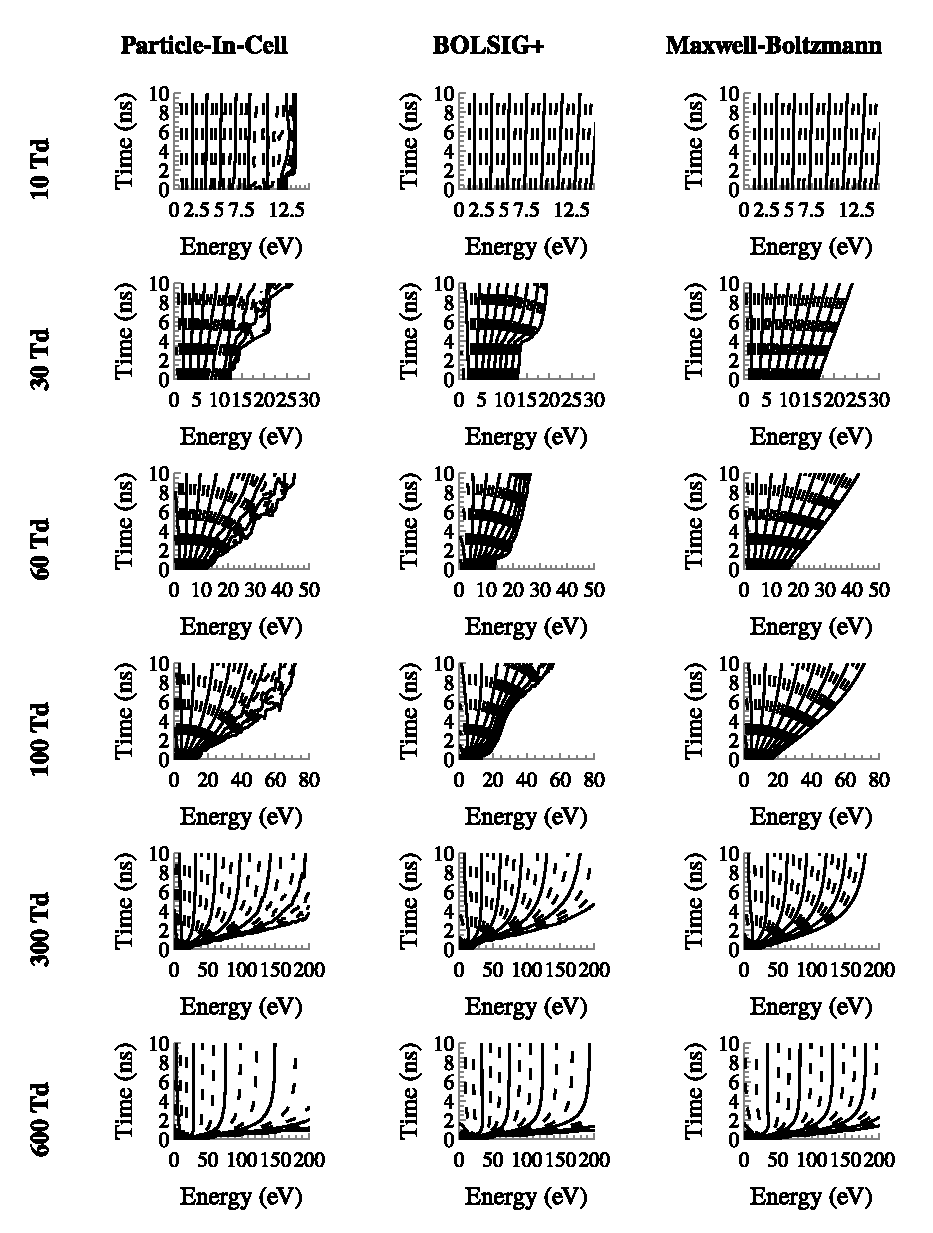
\includegraphics{./chapters/modeling/figures/picmb.eps}
  \caption{Contour plots of the \acs{eedf}s determined from \acs{pic}
    simulations, and the corresponding Maxwell-Boltmzann distributions for a range
    of electric fields.}
  \label{fig:picmb}
\end{figure}
as a series of contour plots. The observable jaggedness in the \acs{pic}
contours is due to the the finite number of particles in the system. As can be
seen, the probability density contours generated by the \acs{pic} simulations
and the corresponding Maxwell-Boltzmann distributions are extremely similar for
electric fields of 100 Td or below. The two approaches begin to deviate from
each other once the field reaches 300 Td. The \acs{eedf}s generated by the
\acs{pic} simulations exhibit a larger number of electrons at low energies (less
than 20 eV) and high energies (greater around 100 eV).

The differences at the high fields can be traced back to the form of the helium
cross sections used in XPDP1. The only reactions available to electrons in the
simulation are elastic scattering, excitation (19.6 eV threshold), and
ionization (24.6 eV threshold). This results in a electron population which is
depleted above these threshold values. The cross sections for these reaction
peak at about four times the threshold energy, thus electrons with energies
in excess of 100 eV are more prevalent. To some extent, these differences would
be lessened in a real discharge. Excited helium offers a number of reactions
with lower threshold energies. However, this depends on the prevalence of
excited helium states.



\subsection{Energy Equation}



\section{Pulse Shape}



\section{Plasma Parameters}



\section{Summary}



